% arara: pdflatex
% arara: pdflatex
% arara: pdflatex

% options:
% thesis=B bachelor's thesis
% thesis=M master's thesis
% czech thesis in Czech language
% slovak thesis in Slovak language
% english thesis in English language
% hidelinks remove colour boxes around hyperlinks

\documentclass[thesis=M,czech]{FITthesis}[2019/03/06]

\usepackage[utf8]{inputenc} % LaTeX source encoded as UTF-8
\usepackage{float}
\usepackage{subfig}
\usepackage{enumitem}

\usepackage{newfloat}
\DeclareFloatingEnvironment[placement={!ht},name=Seznam]{mylist}
% \usepackage{amsmath} %advanced maths
% \usepackage{amssymb} %additional math symbols

\usepackage{dirtree} %directory tree visualisation

% % list of acronyms
% \usepackage[acronym,nonumberlist,toc,numberedsection=autolabel]{glossaries}
% \iflanguage{czech}{\renewcommand*{\acronymname}{Seznam pou{\v z}it{\' y}ch zkratek}}{}
% \makeglossaries

\newcommand{\tg}{\mathop{\mathrm{tg}}} %cesky tangens
\newcommand{\cotg}{\mathop{\mathrm{cotg}}} %cesky cotangens

% % % % % % % % % % % % % % % % % % % % % % % % % % % % % % 
% ODTUD DAL VSE ZMENTE
% % % % % % % % % % % % % % % % % % % % % % % % % % % % % % 

\department{Katedra \ldots softwarového inženýrství}
\title{MIDI stage piano}
\authorGN{Petr} %(krestní) jméno (jména) autora
\authorFN{Svoboda} %príjmení autora
\authorWithDegrees{Bc. Petr Svoboda} %jméno autora vcetne soucasných akademických titulu
\author{Petr Svoboda} %jméno autora bez akademických titulu
\supervisor{Ing. Josef Pavlíček, Ph.D.}
\acknowledgements{Doplnte, máte-li komu a za co dekovat. V~opacném prípade úplne odstrante tento príkaz.}
% TODO
\abstractCS{V~nekolika vetách shrnte obsah a prínos této práce v~ceštine. Po prectení abstraktu by se ctenár mel mít ctenár dost informací pro rozhodnutí, zda chce Vaši práci císt.}
\abstractEN{Sem doplnte ekvivalent abstraktu Vaší práce v~anglictine.}
\placeForDeclarationOfAuthenticity{V~Praze}
% TODO
\declarationOfAuthenticityOption{4} %volba Prohlášení (císlo 1-6)
\keywordsCS{VST, MIDI, OSC}
\keywordsEN{VST, MIDI, OSC}
% \website{http://site.example/thesis} %volitelná URL práce, objeví se v tiráži - úplne odstrante, nemáte-li URL práce

\begin{document}

% \newacronym{CVUT}{{\v C}VUT}{{\v C}esk{\' e} vysok{\' e} u{\v c}en{\' i} technick{\' e} v Praze}
% \newacronym{FIT}{FIT}{Fakulta informa{\v c}n{\' i}ch technologi{\' i}}

\begin{introduction}
V hudební branži se můžeme setkat s rozličnými hudebními nástroji. V posledních desetiletích
zaujaly významné místo na trhu elektronické hudební nástroje. Zároveň se s příchodem dostupných a výkonných
výpočetních jednotek začaly objevovat virtuální hudební nástroje\cite{kogan2008brief}.
Jedná se o software, který dokáže generovat zvukovou vlnu v reálném čase na základě kofigurovatelných parametrů a vstupů, jako jsou MIDI data, či zvukový signál.
Lze tak dosáhnout věrné simulace syntezátorů, varhan a dalších mnoha hudebních nástrojů, včetně efektů.
Takové nástroje velmi často implementují některé z dostupných API tak, aby je bylo možné použít v různých prostředích.
Dříve byly hlavní doménou virtuálních nástrojů prostředí pro studiovou produkci hudby\cite{leider2004digital}.
V dnešní době, kdy mobilní zařízení dokáží poskytnout dostatečný výkon, stoupá zájem o využití softwarových hudebních nástrojů
při živých vystoupeních. Cílem práce je navrhnout takové řešení, které by umělci poskytovalo dostatečné možnosti a komfort 
pro efektivní využití virtuálních hudebních nástrojů na pódiu.
	%sem napište úvod Vaší práce
\end{introduction}

\chapter{Analýza}
	\section{Požadavky}
		Z praktických zkušeností lze formulovat následující požadavky na řešení, které bude vyhovovat účelu profesionálního živého vystoupení.
		Jelikož lze požadavky formulovat pouze na obecné úrovni, následuje jejich bodové vyjádření.
		
		Funkční požadavky:
		\begin{itemize}
			\item Ovládací prvky musí být snadno dostupné.
			\item Ovládací prvky musí být precizně ovladatelné.
			\item Uživatel musí být schopen určit aktuální stav systému vizuálním vjemem.
			\item Uživatel může definovat svojí sadu zvuků.
			\item Uživatel může přepínat zvuky z přednastavené sady.
			\item Uživatel může ovládat parametry zvuku v reálném čase.
			\item Uživatel může uložit aktuální zvuk.
			\item Uživatel může ovládat bězné parametry systému, jako např. hlasitost, transpozice.
		\end{itemize}
	
		Nefunkční požadavky:
		\begin{itemize}
			\item Systém nesmí přestat reagovat.
			\item Systém nesmí generovat nežádoucí zvuky.
			\item Systém musí správně ukládat konfiguraci poskytnutou uživatelem.
			\item Systém nesmí umělce omezovat dlouhou dobou prodlevy.
		\end{itemize}
		
	\section{Průzkum existujících řešení}
		\subsection{Hardwarové nástroje}
			Mezi hardwarovými hudebními nástroji se lze setkat s různou mírou optimalizace pro živá vystoupení.
			Zde budeme uvažovat pouze skupinu nástrojů, která je tomuto účelu nejblíže, tzv. stage piana.
			
			Tyto nástroje často poskytují obsáhlou banku zvuků, propracované uživatelské rozhraní a velmi vysokou stabilitu.
			Pokročilejší modely disponují možností přidat nové zvuky v proprietárním formátu, které může uživatel vytvořit za pomocí speciálního nástroje,
			nebo je získat z online databáze. Některé modely navíc umožňují připojit další klaviaturu přes MIDI rozhraní, to ovšem přináší jistá omezení,
			například absenci možnosti použít zvuk stejného typu na obou klaviaturách současně, jelikož zařízení disponuje pouze jedním zvukovým modulem
			pro daný typ zvuku.
			Zároveň nástroje poskytují bohaté možnosti nastavení běžných parametrů, jako jsou např. hlasitost, transpozice, rozdělení klaviatury do zón,
			citlivost klaviatury apod.
			
			Typickým zástupcem jsou modely značky Nord (obr. \ref{fig:HardwareStagepiano}), které jsou velmi oblíbené pro svoji stabilitu a mnohostrannost, jsou nicméně poměrně nákladnou záležitostí.
			
			\begin{figure}[H]
				\centering
				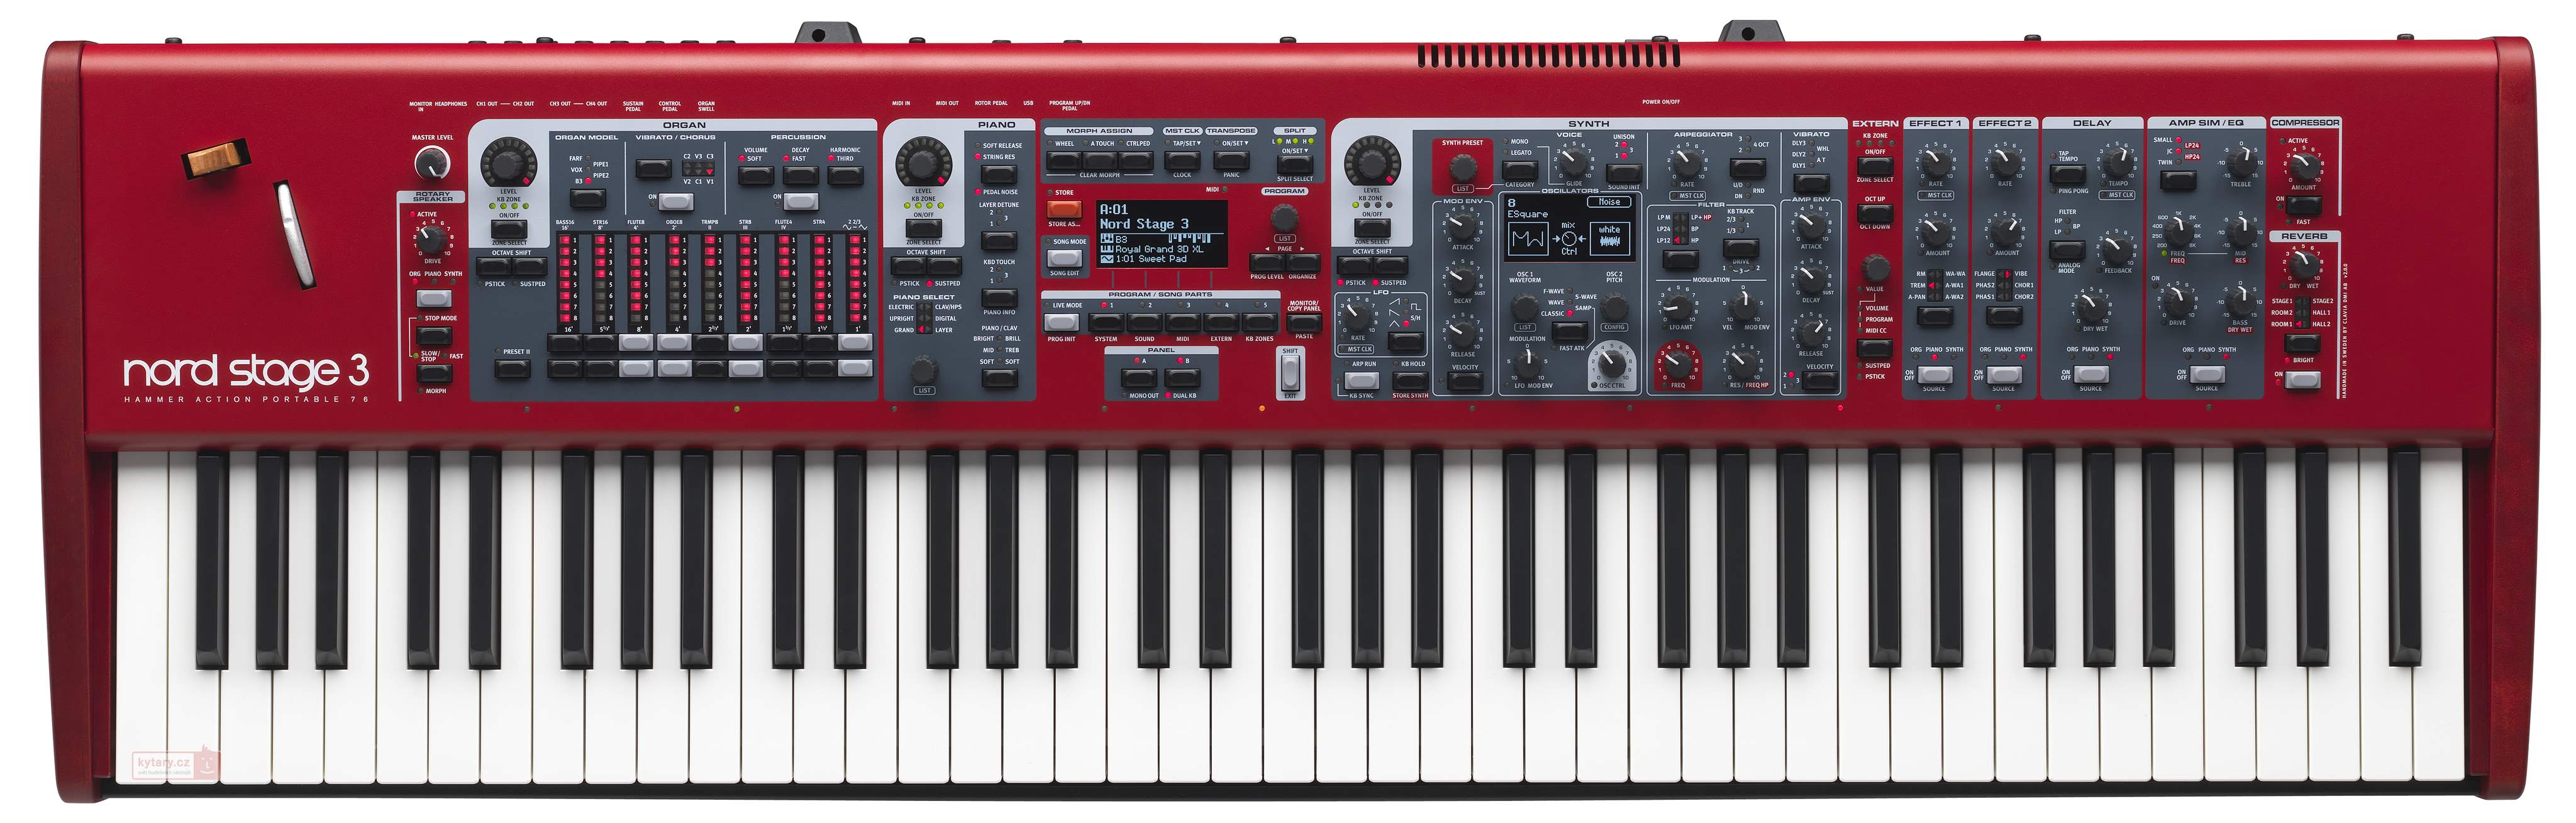
\includegraphics[width=1\textwidth]{HardwareStagepiano}
				\caption[Nord Stage 3 HP]{Nord Stage 3 HP}\label{fig:HardwareStagepiano}
			\end{figure}
		\subsection{Prostředí typu DAW}
			Prostředí typu DAW jsou určena převážně pro studiovou práci, tedy nahrávání, střih, míchání a postprodukci zvukového materiálu.
			K jejich využití je potřeba počítač nebo tablet. Klaviatury jsou připojeny přes MIDI rozhraní. Ke generování zvuku používají virtuální hudební nástroje.
			V prostředí lze používat více stop, kde každá stopa může používat různý virtuální nástroj a sadu efektů.
			Poskytuje také bohaté možnosti routování zvukového signálu.
			Nechybí ani integrace s klaviaturami a kontrolery, což usnadňuje práci a přispívá ke komfortu užívání.
			
			Ikdyž je prostředí typu DAW primárně určeno pro studiovou práci, může být vhodné i pro použití při živých vystoupeních.
			Jedná se však převážně o takový typ vystoupení, kdy má umělec předem pečlivě připravené celé představení.
			Flexibilita prostředí při samotném vystoupení je pak nízká.
			Lze sice docílit i flexibilního chování, nezbytná je však interakce uživatele s počítačem, nebo tabletem. Při živém vystoupení
			je však taková interakce značně nevhodná, jelikož neposkytuje dostatečnou rychlost a preciznost ovládání.
			Navíc lze použít pouze omezené množství přednastavených zvuků, jelikož pro každý zvuk musí být zavedena zvláštní instance
			virtuálního nástroje, která čerpá systémové prostředky.
			
			\begin{figure}[H]
				\centering
				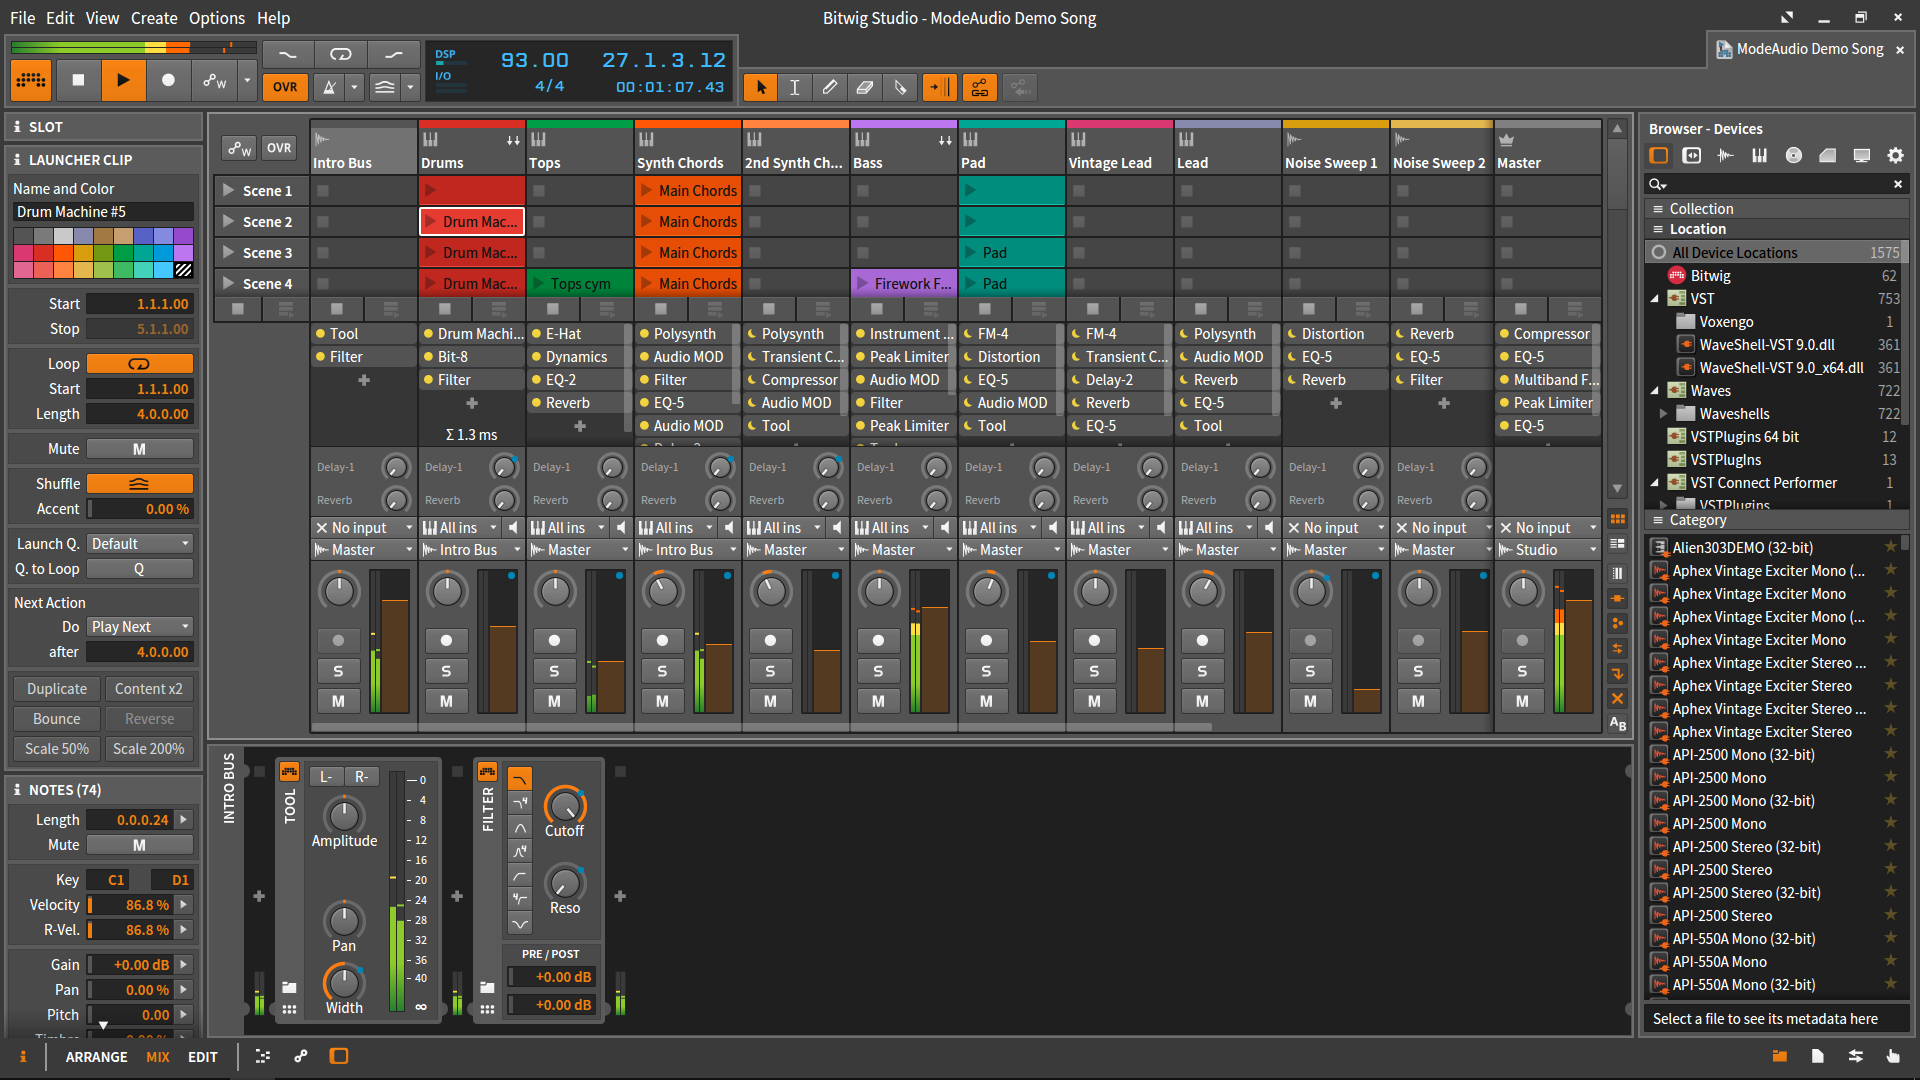
\includegraphics[width=1\textwidth]{DAW}
				\caption[Bitwig Studio]{Ukázka prostředí Bitwig Studio}\label{fig:DAW}
			\end{figure}
			
\clearpage
		\subsection{Prostředí pro živá vystoupení}
			S příchodem výkonných mobilních zařízení se začaly objevovat prostředí pro živá vystoupení.
			Poněvadž jde o novou oblast a uživatelská základna není příliš početná, každé řešení přichází
			s unikátním přístupem. Následuje výčet vlastností, které jsou pro většinu takových řešení společné.
			
			\begin{itemize}
				\item Snaha o optimalizaci využití systémových prostředků.
				\item Možnost vkládat vlastní skladby a jejich části.
				\item Možnost uložit konfiguraci zvuku pro skladbu a její část.
				\item Přítomnost filtrů, transformací a směrování MIDI zpráv.
				\item Podpora ovládání prostředí hardwarovým kontrolerem nebo tabletem.
				\item Multiplatformní podpora
				\item Podpora VST/VSTi API
			\end{itemize}
		
			V následující podkapitole bude zkoumán přední představitel prostředí pro živá vystoupení,
			software Cantabile od společnosti Topten Software.
			
			\subsubsection{Prostředí Cantabile}
				Software Cantabile od společnosti Topten Software představuje robustní řešení.
				Implementuje pokročilé optimalizace využití systémových prostředků a
				disponuje širokými možnostmi konfigurace, ovládání však není příliš intuitivní. (obr. \ref{fig:Cantabile})
				Prostředí umožňuje použití více klaviatur, jejich rozdělení na zóny a poskytuje bohaté možnosti
				pro směrování a transformaci MIDI zpráv, což zajišťuje vysokou flexibilitu.
				Způsob ukládání nastavení VST pluginů poskytuje více strategií.
				Cantabile se opírá o model uložení konfigurace pro uživatelem zadanou skladbu nebo její část.
				Integrace s hardwarovými kontrolery je z pohledu vstupu na vysoké úrovni, ovládacím prvkům lze přiřadit jakoukoliv 
				funkci programu. Z hlediska výstupu je však integrace omezená na obecnou úroveň, pro efektivní použití
				je třeba používat zároveň tablet nebo počítač.
				\begin{figure}[H]
					\centering
					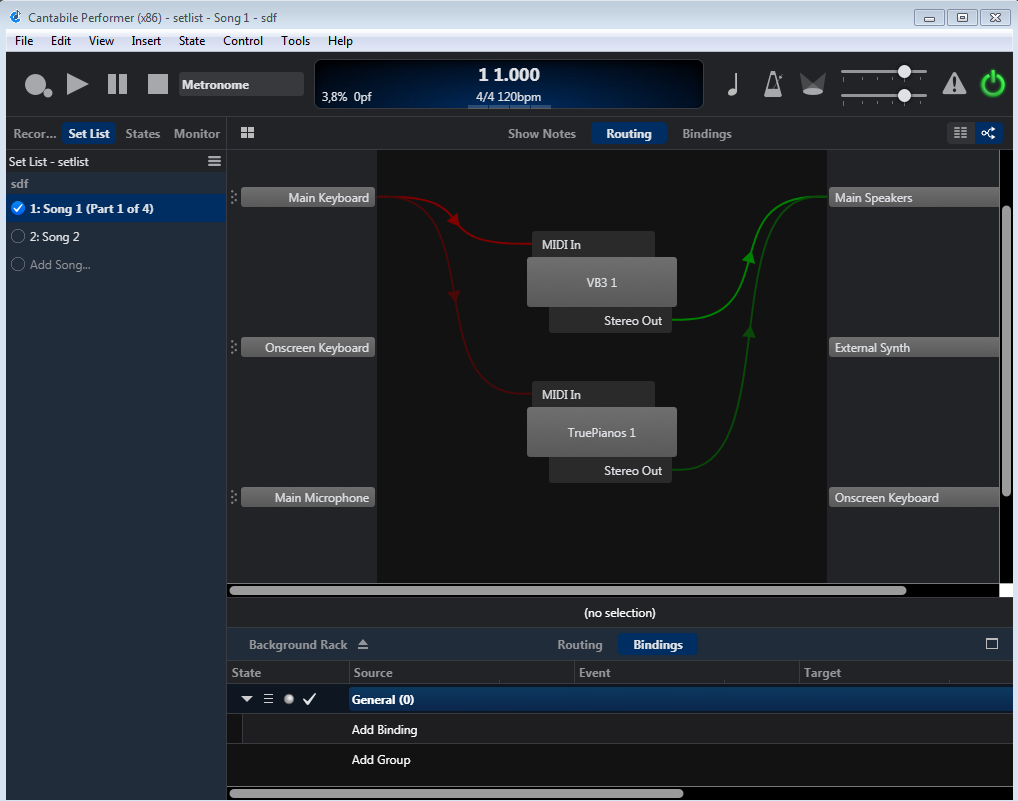
\includegraphics[width=1\textwidth]{Cantabile}
					\caption[Bitwig Studio]{Ukázka prostředí Cantabile}\label{fig:Cantabile}
				\end{figure}
		
	\section{Závěr}
		Z provedeného průzkumu plyne, že existují různé možnoti řešení. Každé z nich řeší problém různým způsobem a má své výhody a nevýhody.
		Nebylo však nalezeno řešení, které by přinášelo možnost využití virtuálních hudebních nástrojů a integraci s hardwarovým kontrolerem tak,
		aby bylo dosaženo chování hardwarových hudebních nástrojů. Proto byla zvolena cesta návrhu vlastního řešení.

\chapter{Návrh vlastního řešení}
	\section{Architektura}
		Jelikož by bylo zbytečné realizovat celé řešení, bylo použito vzájemné propojení více technologií tak,
		aby vlastní implementace řešila pouze problémy přímo související s dosažením kýženého chování systému. V následujících podkapitolách
		budou rozebrány jednotlivé části architektury.
		
		\subsection{VST host}
			Každý virtuální hudební nástroj podporující VST API\cite{vstdoc}, tzv. VST plugin, potřebuje ke svému běhu hostitelské prostředí, tzv. VST host aplikaci, která API implementuje\cite{vstdoc}.
			
			VST API umožňuje pluginům generovat zvukovou vlnu na základě konfigurovatelných
			parametrů a vstupních dat, jako jsou MIDI události, či zvukový signál.
			Konfigurace parametrů virtuálního nástroje probíhá přes vlastní uživatelské rozhraní pluginu, nebo přes hostitelskou aplikaci.
			Každý VST plugin poskytuje hostitelské aplikaci výčet dostupných parametrů a jejich vlastnosti.
			Zároveň je připravena i podpora tzv. presetů, které reflektují stav pluginu. Presety lze ovládat též prostřednictvím
			hostitelské aplikace.
			
			Hostitelská aplikace zároveň zajišťuje přenos zvukového signálu z pluginu, např. do zvukového rozhraní zařízení,
			a přenos MIDI zpráv do pluginu, např. z připojené klaviatury či kontroleru. Hostitelská aplikace musí vykazovat
			vysokou stabilitu, aby nedocházelo k výpadkům ve streamu zvukového signálu či k zahazování MIDI zpráv. Oblíbenou 
			technologií používanou k implementaci ovladačů zvukových zařízení při zachování nízké latence je technologie ASIO\cite{asio}.
			
			Jelikož by byla implementace funkcí hostitelského prostředí náročnou záležitostí, byl zvolen přístup využití
			již existující aplikace, která bude plnit úlohu VST hostitelského prostředí a bude ovládána externě naší vlastní aplikací.
			
		\subsection{OSC}		
			OSC představuje obecný a jednoduchý protokol určený pro přenos zpráv mezi multimediálními zařízeními a aplikacemi\cite{osc}.
			Zprávy jsou přenášeny typicky přes UDP protokol. Multimediální aplikace často poskytují možnost oboustranné integrace
			se službami třetích stran právě přes OSC protokol.

		\subsection{HW kontroler}
			Hardwarový kontroler slouží k ovládání multimediálních aplikací nebo zařízení. V naprosté většině případů k přenosu používá MIDI protokol
			a bývá připojen přes rozhraní USB nebo MIDI. Kontroler navíc může být vybaven prezentačními prvky, jako jsou LED indikátory, display apod.

		\subsection{Automap}
			Protokol Automap od společnosti Novation je postavený nad protokolem MIDI, využívá kombinaci zpráv typu CC a SysEx \cite{midi}\cite{automap}.
			Slouží k integraci multimediálních aplikací se skupinou kontrolerů od společnosti Novation. Existují implementace pro 
			přední DAW prostředí.

		\subsection{Vlastní aplikace}
			Cílem vlastní aplikace je propojení všech komponent tak, aby bylo dosaženo požadované funkcionality.
			Aplikace bude ovládat VST hostitelské prostředí a v něm obsažené nástroje a efekty s využitím OSC protokolu.
			S hardwarovým kontrolerem bude aplikace obousměrně integrována přes protokol Automap.
			K dispozici bude též desktopové uživatelské rozhraní sloužící ke konfiguraci zvuků, presetů a dalších nastavení.
\clearpage
		\subsection{Závěr}
			Na diagramu \ref{fig:Architecture} je zobrazena architektura systému.
			\begin{figure}[H]
				\centering
				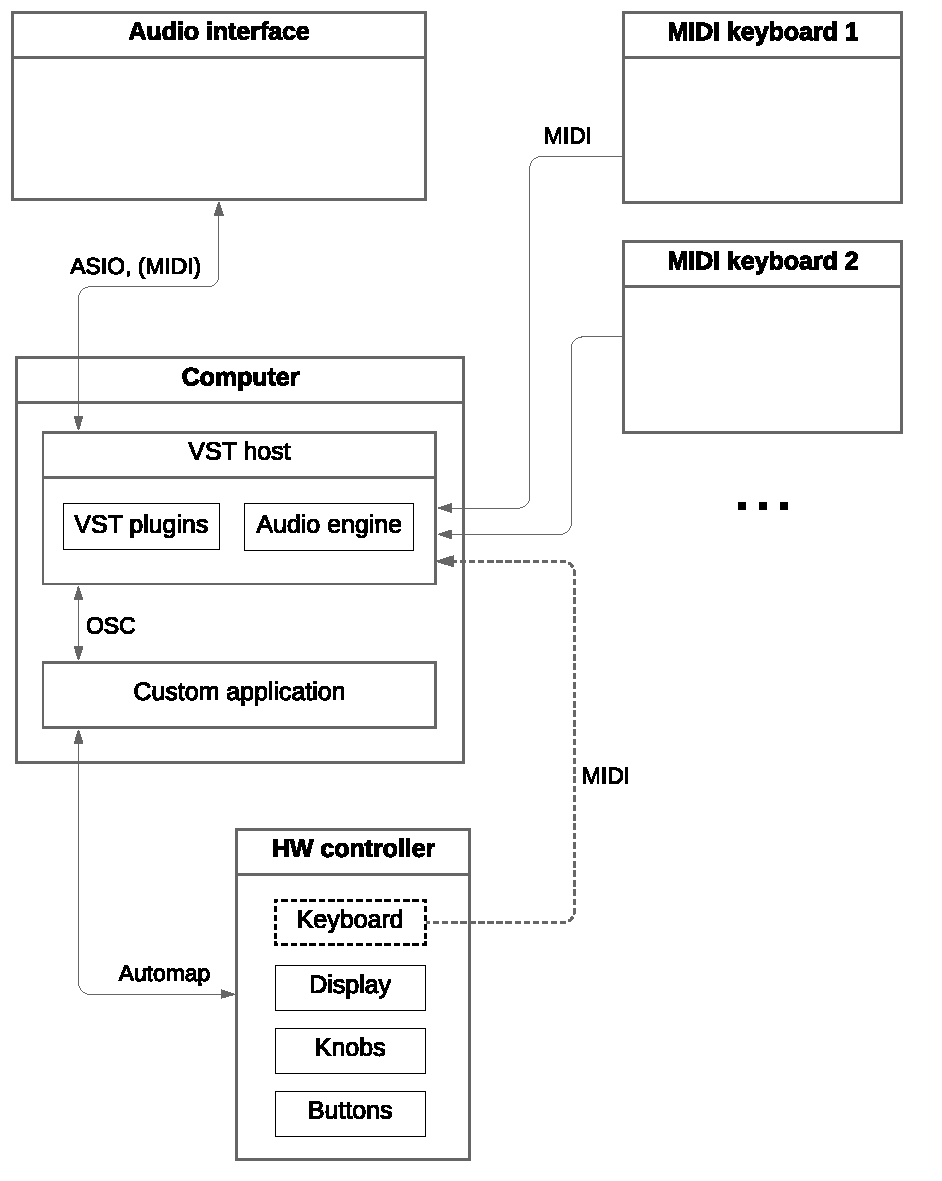
\includegraphics[width=1\textwidth]{Architecture}
				\caption[Architektura řešení]{Architektura řešení}\label{fig:Architecture}
			\end{figure}
\clearpage
	\section{Analýza kompatibility}
		Na počátku byla provedena analýza kompatibility jednotlivých komponent. 
		
		\subsection{HW kontroler}
		Při analýze kompatibility kontroleru za použití modelu Novation SLMkII 49 bylo zjištěno, že
		kontroler připojený přes USB sice exportuje rozhraní pro komunikaci přes protokol Automap,
		ale toto rozhraní nehlásí systému příslušnou třídu USB zařízení. Podle zachycené sériové komunikace
		se ukázalo, že formát přenášených dat přesto odpovídá třídě USB pro MIDI zařízení\cite{usbmidi}.
		
		\subsection{VST host}
		Jako hostitelská aplikace pro VST pluginy byl testován program Bidule of společnosti Plogue.
		Z anlýzy vyplynulo, že poskytuje bohaté možnosti ovládání přes kombinaci protokolů OSC a UDP.
		Program přes OSC umožňuje spouštět důležité akce, lze navíc přijímat a odesílat hodnoty všech VST pluginů a interních modulů.
		Data jsou uložena ve formátu XML, ze kterého lze snadno získat veškeré informace o uloženém projektu.
		
	\section{Zvolené technologie}
		Na základě analýzy kompatibility byl jako hardwarový kontroler zvolen model Novation SLMkII 49, jako VST hostitelskou aplikací byl zvolen program Bidule od společnosti Plogue.
		Pro zajištění nízkoúrovňové komunikace s kontrolerem byl zvolen univerzální USB ovladač WinUSB pro platformu Windows.
	
		Při výběru technologií pro implementaci vlastní aplikace byly zohledněny následující požadavky:
		\begin{itemize}
			\item Možnost low-level komunikace přes USB
			\item Podpora komunikace přes UDP
			\item Podpora asynchronního kódu na vysoké úrovni
			\item Nenáročná tvorba UI
			\item Stabilita a rychlost odezvy
		\end{itemize}
			
		Pro implementaci vlastní aplikace byl zvolen programovací jazyk TypeScript, jehož kód je kompilován do jazyka JavaScript.

		Dále byl zvolen framework Electron, který poskytuje možnost tvorby desktopových aplikací za použití jazyka JavaScript.
		Při spuštění aplikace vytvořené ve frameworku Electron je spuštěn na pozadí tzv. hlavní proces.
		Hlavní proces vytváří další vedlejší nezávislé procesy, které slouží k zobrazení oken s webovým prohlížečem, kde je načtena klientská část aplikace.
		Ke komunikaci mezi hlavním a vedlejšími procesy framework poskytuje jednoduché rozhraní.

		Jelikož lze komunikaci mezi aplikací a hardwarovým kontrolerem implementovat pouze v hlavním procesu, bylo původním záměrem využítí architektonického vzoru tlustý klient. 
		Hlavní proces by fungoval pouze jako proxy pro protokoly OSC a Automap mezi příslušnými komponentami a klientskou částí aplikace (diagram \ref{fig:AppArchitectureA}).
		Při testování bylo zjištěno, že rozhraní pro komunikaci mezi hlavním a vedlejšími vlákny není pro tento účel dostatečně rychlé a nemá dostatečně rychlou odezvu.
		Jako řešení tohoto problému bylo zvoleno rozdělení aplikace na serverovou a klientskou část, kde mezi oběmi stranami nebude docházet k objemné komunikaci citlivé na dobu odezvy.
		Jelikož lze předpokládat, že velká část stavu aplikace bude sdílená serverovou i klientskou částí, byl vybrán pro obě části framework pro vývoj webových aplikací Angular a knihovna NGXS představující framework pro řízení stavu podle patternu CQRS\cite{cqrs}, který vychází ze vzoru CQS\cite{cqs}. Výhodou je pak možnost automatické synchronizace stavu mezi serverovou a klientskou částí (diagram \ref{fig:AppArchitectureB}).
		



		\begin{figure}
			\centering
%			\parbox{5cm}{
%				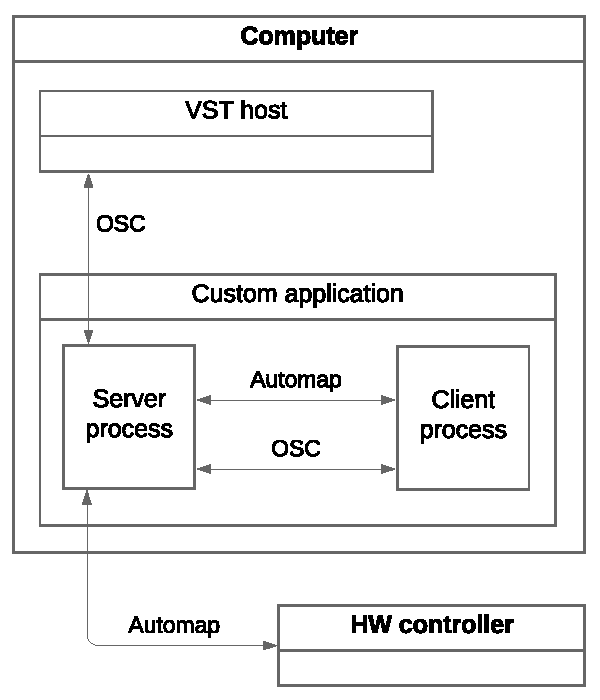
\includegraphics[width=5.5cm]{Dip-AppArchitecture1}
%				\caption{Původní návrh architektury aplikace.}
%				\label{fig:AppArchitectureA}}
%			\qquad
%			\begin{minipage}{5cm}
%				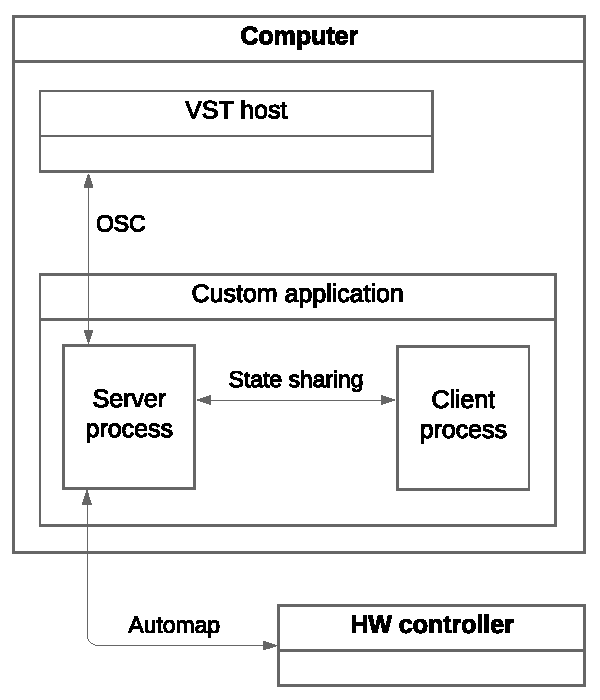
\includegraphics[width=5cm]{Dip-AppArchitecture2}
%				\caption{Optimalizovaný návrh architektury.}
%				\label{fig:AppArchitectureB}
%			\end{minipage}
			
			\subfloat[Původní návrh]{{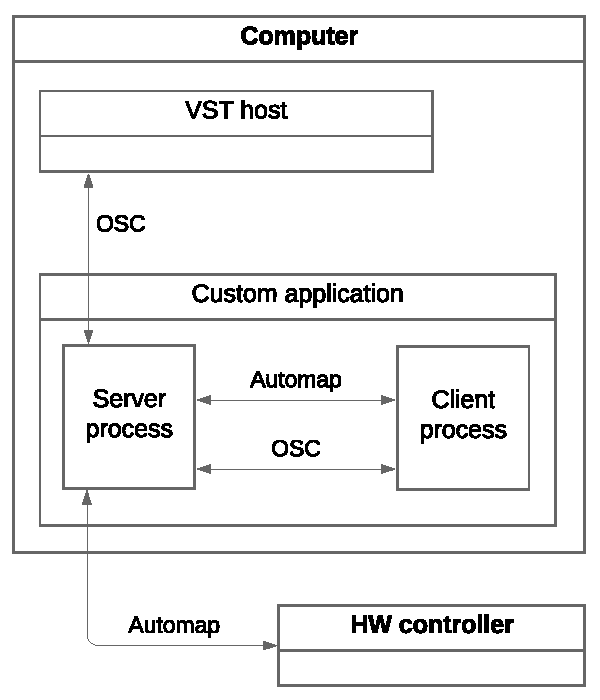
\includegraphics[width=5.8cm]{Dip-AppArchitecture1}								\label{fig:AppArchitectureA} }}
			\qquad
			\subfloat[Optimalizovaný návrh]{{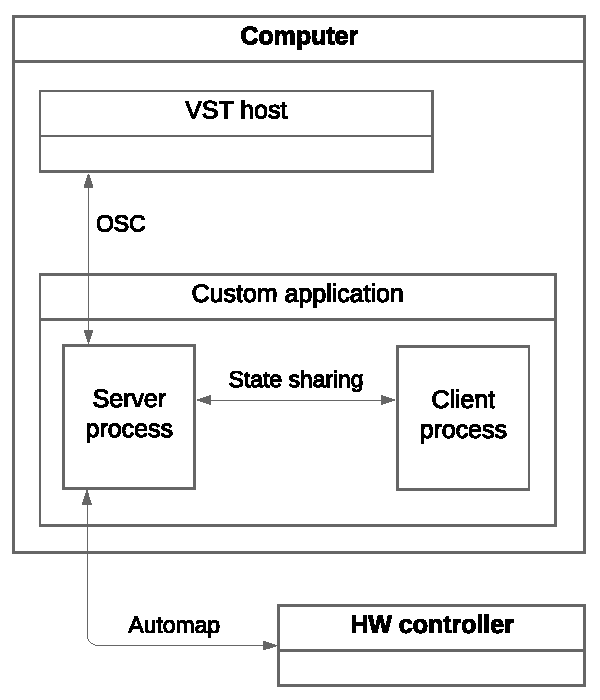
\includegraphics[width=5.8cm]{Dip-AppArchitecture2}
				\label{fig:AppArchitectureB} }}
			\caption{Srovnání původního a konečného návrhu architektury aplikace.}
			\label{fig:AppArchitecture}
		\end{figure}
		
		Pro klientskou část byla použita knihovna \texttt{Angular Material UI}, která poskytuje základní prvky pro tvorbu uživatelského rozhraní.

		Pro servrovou část byla využita knihovna \texttt{tessel/node-usb}, jejíž úlohou je zpřístupnění funkcí knihovny \texttt{libusb}\cite{libusb}, která poskytuje možnost low-level komunikace s USB zařízeními.
		V serverové části též byla využita knihovna \texttt{node-osc}, která umožňuje komunikaci přes OSC a UDP protokol.
		
	\section{Funkční požadavky}
		Při návrhu řešení byly určeny následující funkční požadavky.
	
		V aplikaci bude možné používat více projektů programu Bidule. Bude k dispozici rozhraní pro správu projektů, kde bude možné
		zadat cestu k uloženému projektu a název projektu. Je možné načíst a zavřít projekt. Veškerá nastavení kromě globálních se budou ukládat 
		pro každý projekt zvlášť. Po načtení projektu dojde k automatickému importu konfigurace projektu Bidule.
		
		Vrstvou se rozumí skupina VST pluginů definovaná v projektu programu Bidule. Manuálem se rozumí skupina vrstev a představuje připojenou klaviaturu.

		V rámci aplikace bude možné zobrazit seznam dostupných nástrojů a efektů. Seznam nástrojů a efektů bude importován z konfigurace projektu Bidule.
		U nástrojů a efektů bude možné vytvořit snímek všech parametrů pluginu, který bude považován za výchozí a bude načten při načtení projektu, nebo po přepnutí zvuku. V rámci obou seznamů bude též možné otevřít uživatelské rozhraní VST pluginu, či zobrazit jeho dostupnost v jednotlivých vrstvách. Pro nástroje bude možnost definovat více pojmenovaných stránek mapování, pro efekt bude možné zadat právě jednu stránku mapování s volbou hlavního mapování.

		Editor stránek mapování bude poskytovat možnost konfigurace mapování parametrů VST pluginu na enkodery kontroleru.
		V rámci jedné stánky mapování bude možné ke každému enkoderu přiřadit právě jeden parametr VST pluginu a zadat tak až 8 různých mapování.
		Při volbě parametru pluginu bude možné použít tzv. funkce learn, kdy lze ovládaný parametr vybrat přímo v uživatelském rozhraní pluginu.
		Bude možné zadat název mapování.
		Pro každé mapování budou k dispozici následující strategie:
		\begin{itemize}
			\item\label{LinearMappingStrategy} \textbf{Lineární} - Tato strategie bude umožňovat určit lineární vztah mezi hodnotou enkodéru na hardwarovém kontroleru 
			a hodnotou parametru příslušného pluginu. Bude možné zadat rozsah hodnot zobrazených na displayi, rozsah hodnot parametru VST pluginu, invertovat
			průběh a zadat suffix pro zobrazení na displayi. Rozsah hodnot parametrů pluginu bude možné nastavovat i přes tzv. learn metodu, která 
			umožňuje hodnoty zvolit přímo v prostředí VST pluginu. Na LED prstencích otočných enkodérů kontroleru bude hodnota parametru indikována lineárně na celém rozsahu enkodéru.
			
			\item \textbf{Lineární s položkovým zobrazením} - Jedná se o rozšíření Lineární strategie rožšířené o možnost zadání položek, které
			budou zobrazeny na displayi v závislosti na hodnotě parametru pluginu. Každá položka bude určena názvem a hraniční hodnotou parametru VST pluginu.
			Položky bude možné přidávat i za pomoci tzv. learn metody, kdy je možné zadat hraniční hodnotu přímo v prostředí VST pluginu.

			\item \textbf{Seznam} - Za použití této strategie bude možné definovat seznam položek obsahujících název a hodnotu parametru VST pluginu.
			Oproti lineární strategii s položkovým zobrazením bude probíhat změna hodnoty parametru VST pluginu skokově. Při reflektování změn hodnoty parametru bude zobrazena
			položka, která je aktuální hodnotě parametru nejblíže.
		\end{itemize}
		
		V editoru presetů bude možné zadat až 8 kategorií zvuků, které bude možné řadit a přejmenovat.
		Pro každou kategorii bude možné přidat nový preset, či duplikovat stávající. Preset určuje použitý VST plugin,
		strategii inicializace pluginu vč. její konfigurace, rozdílovou sadu hodnot parametrů pluginu a rozdílovou sadu hodnot parametrů efektů vrstvy.
		Rozdílová sada bude pro danou vrstvu vytvářena při změně v parametrech pluginu v době, kdy je plugin aktivní. Zaznamenanou sadu bude možné pro aktivní preset uložit.
		V rámci inicializace VST pluginu budou k dispozici následující strategie:
		\begin{itemize}
			\item \textbf{Snímek všech parametrů} - V této strategii bude možné pořídit snímek hodnot všech parametrů VST pluginu. Snímek bude načten při načtení presetu.
			\item Zpráva typu Program Change - Tato strategie zajistí odeslání MIDI zprávy typu Program Change do patřičného VST pluginu.
			\item Načtení nativního VST presetu - Za použití této strategie dojde k načtení nativního presetu VST pluginu. Nativní presety je možné editovat
			v hostitelské aplikaci či přímo v pluginu.
		\end{itemize}
		Pro každou vrstvu může být aktivní právě jeden preset. Po načtení presetu bude 
		pro danou vrstvu aplikovaná inicizalizační strategie na virtuální nástroj a budou načteny rozdílové sady hodnot parametrů nástroje a efektů.
		Vlastnosti presetu bude možné upravit, či preset odstranit.
	
		Za použití kontroleru bude možný výběr kategorie a stránkovaný výběr presetu v rámci dané kategorie. Zároveň bude k dispozici
		historie posledních použitých presetů vč. jejich stavů pro každou vrstvu.
		Hodnoty parametrů pluginů bude možné ovládat otočnými enkodéry kontroleru. Hodnoty budou indikovány LED prstencem enkodéru a grafickým výstupem na displayi podle konfigurace strategie mapování.
		V rámci ovládání parametrů nástrojů bude k dispozici
		zobrazení stránky mapování daného presetu. Pro ovládání parametrů efektů bude k dispozici agregované zobrazení, kde bude zobrazena
		hlavní položka stránky mapování pro každý efekt, který je v dané vrstvě dostupný. Bude možné ovládat i všechny parametry efektu.
		Kontroler uživateli umožní přepínat a indikovat právě ovládanou vrstvu. 
		Za pomocí posuvných prvků kontroleru bude možné ovládat hlasitosti jednotlivých vrstev.
		K dispozici bude též ovládání hlavní hlasitosti a tzv. funkce Panic pro ukonćení všech znějících tónů.
	
	\section{Doménový model}
		Z analýzy požadavků byl navržen doménový model (\ref{obr. fig:DomainModel}),
		který modeluje entity problémové domény a jejich vzájemné vztahy.
		\begin{figure}
			\centering
			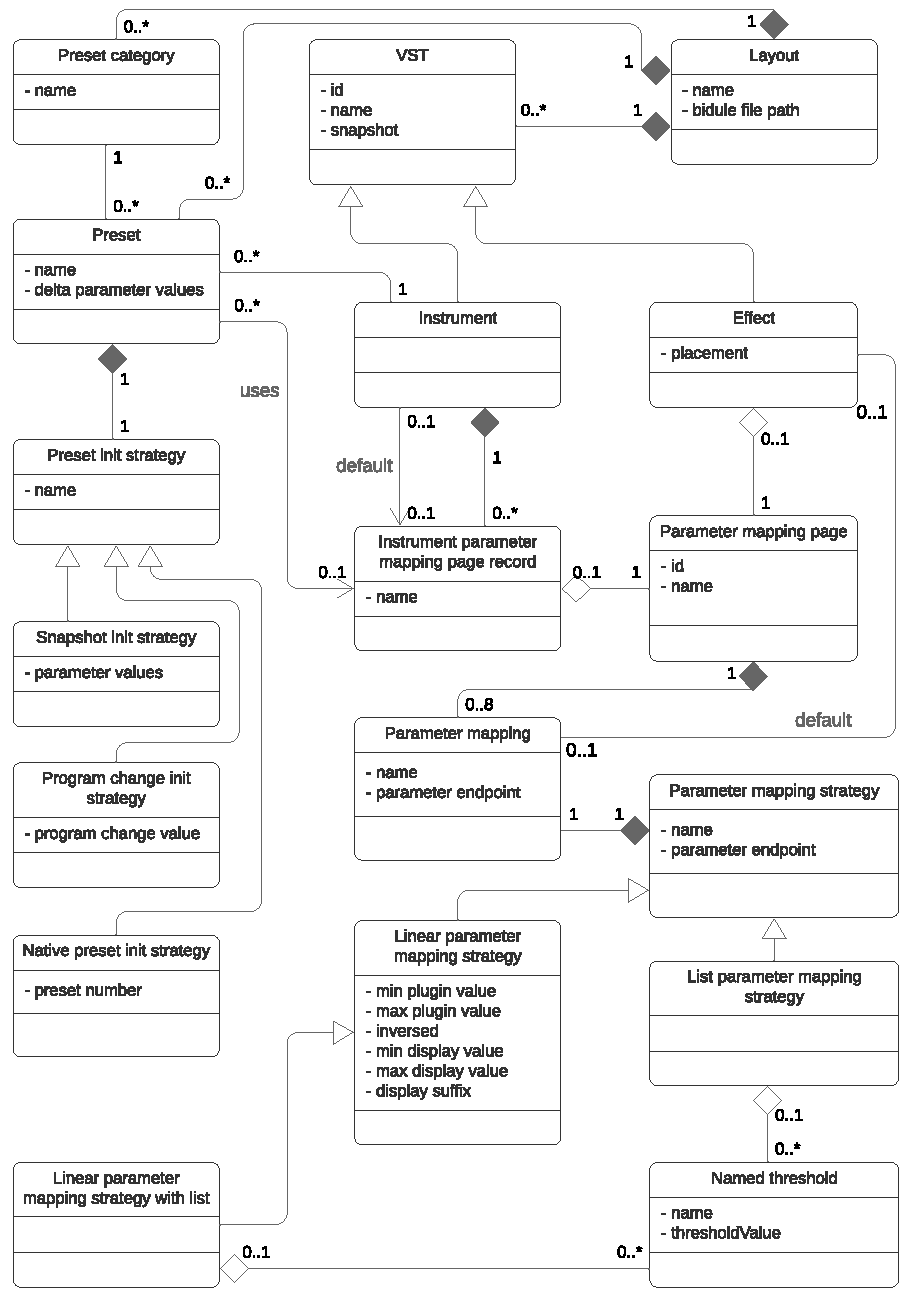
\includegraphics[width=1\textwidth]{DomainModel}
			\caption[Doménový model]{Doménový model}\label{fig:DomainModel}
		\end{figure}		

	\section{Desktopové uživatelské rozhraní}
		Při návrhu uživatelského rozhraní desktopové aplikace
		byl sestrojen následující seznam obrazovek.
		\begin{mylist}
			\begin{enumerate}[label=\textbf{S\arabic*}]
				\item Seznam projektů
				\item Editace projektu
			\end{enumerate}
			\caption{Seznam obrazovek desktopového uživatelského rozhraní aplikace}\label{list:DesktopUIScreen}		
		\end{mylist}

	\section{Uživatelské rozhraní kontroleru}
		
		
\chapter{Implementace vlastního řešení}
	\section{USB}

		- Implementace midi přes USB

	\section{NGXS}
		
		- Synchronizace
		
		- Stavy
		
	\section{OSC}
	
		- asynchronni zpracovani
		- komunikace s Bidule
	
	\section{Kontroler}
	
		- abstrakce
		- asynchronni
		- model pro tlacitka
		- model pro display
		- model pro dalsi prvky
	
	\section{Desktop UI}
		- angular material
		
	\section{Data}

		- import dat z bidule
		- ukladani dat


\chapter{Testování}

\begin{conclusion}
	%sem napište záver Vaší práce
\end{conclusion}

\bibliographystyle{csn690}
\bibliography{mybibliographyfile}

\appendix

\chapter{Seznam použitých zkratek}
% \printglossaries
\begin{description}
	\item[VST] Virtual studio technology
	\item[VSTi] Virtual studio technology instrument
	\item[API] Application Programming Interface
	\item[DAW] Digital audio workstation
	\item[OSC] Open sound control
	\item[ASIO] Audio streaming input output
	\item[XML] Extensible markup language
	\item[CQRS] Command Query Responsibility Segregation
	\item[CQS] Command Query Separation
\end{description}


% % % % % % % % % % % % % % % % % % % % % % % % % % % % 
% % Tuto kapitolu z výsledné práce ODSTRANTE.
% % % % % % % % % % % % % % % % % % % % % % % % % % % % 
% 
% \chapter{Návod k~použití této šablony}
% 
% Tento dokument slouží jako základ pro napsání záverecné práce na Fakulte informacních technologií CVUT v~Praze.
% 
% \section{Výber základu}
% 
% Vyberte si šablonu podle druhu práce (bakalárská, diplomová), jazyka (ceština, anglictina) a kódování (ASCII, \mbox{UTF-8}, \mbox{ISO-8859-2} neboli latin2 a nebo \mbox{Windows-1250}). 
% 
% V~ceské variante naleznete šablony v~souborech pojmenovaných ve formátu práce\_kódování.tex. Typ muže být:
% \begin{description}
% 	\item[BP] bakalárská práce,
% 	\item[DP] diplomová (magisterská) práce.
% \end{description}
% Kódování, ve kterém chcete psát, muže být:
% \begin{description}
% 	\item[UTF-8] kódování Unicode,
% 	\item[ISO-8859-2] latin2,
% 	\item[Windows-1250] znaková sada 1250 Windows.
% \end{description}
% V~prípade nejistoty ohledne kódování doporucujeme následující postup:
% \begin{enumerate}
% 	\item Otevrete šablony pro kódování UTF-8 v~editoru prostého textu, který chcete pro psaní práce použít -- pokud mužete texty s~diakritikou normálne precíst, použijte tuto šablonu.
% 	\item V~opacném prípade postupujte dále podle toho, jaký operacní systém používáte:
% 	\begin{itemize}
% 		\item v~prípade Windows použijte šablonu pro kódování \mbox{Windows-1250},
% 		\item jinak zkuste použít šablonu pro kódování \mbox{ISO-8859-2}.
% 	\end{itemize}
% \end{enumerate}
% 
% 
% V~anglické variante jsou šablony pojmenované podle typu práce, možnosti jsou:
% \begin{description}
% 	\item[bachelors] bakalárská práce,
% 	\item[masters] diplomová (magisterská) práce.
% \end{description}
% 
% \section{Použití šablony}
% 
% Šablona je urcena pro zpracování systémem \LaTeXe{}. Text je možné psát v~textovém editoru jako prostý text, lze však také využít specializovaný editor pro \LaTeX{}, napr. Kile.
% 
% Pro získání tisknutelného výstupu z~takto vytvoreného souboru použijte príkaz \verb|pdflatex|, kterému predáte cestu k~souboru jako parametr. Vhodný editor pro \LaTeX{} toto udelá za Vás. \verb|pdfcslatex| ani \verb|cslatex| \emph{nebudou} s~temito šablonami fungovat.
% 
% Více informací o~použití systému \LaTeX{} najdete napr. v~\cite{wikilatex}.
% 
% \subsection{Typografie}
% 
% Pri psaní dodržujte typografické konvence zvoleného jazyka. Ceské \uv{uvozovky} zapisujte použitím príkazu \verb|\uv|, kterému v~parametru predáte text, jenž má být v~uvozovkách. Anglické otevírací uvozovky se v~\LaTeX{}u zadávají jako dva zpetné apostrofy, uzavírací uvozovky jako dva apostrofy. Casto chybne uvádený symbol "{} (palce) nemá s~uvozovkami nic spolecného.
% 
% Dále je treba zabránit zalomení rádky mezi nekterými slovy, v~ceštine napr. za jednopísmennými predložkami a spojkami (vyjma \uv{a}). To docílíte vložením pružné nezalomitelné mezery -- znakem \texttt{\textasciitilde}. V~tomto prípade to není treba delat rucne, lze použít program \verb|vlna|.
% 
% Více o~typografii viz \cite{kobltypo}.
% 
% \subsection{Obrázky}
% 
% Pro umožnení vkládání obrázku je vhodné použít balícek \verb|graphicx|, samotné vložení se provede príkazem \verb|\includegraphics|. Takto je možné vkládat obrázky ve formátu PDF, PNG a JPEG jestliže používáte pdf\LaTeX{} nebo ve formátu EPS jestliže používáte \LaTeX{}. Doporucujeme preferovat vektorové obrázky pred rastrovými (vyjma fotografií).
% 
% \subsubsection{Získání vhodného formátu}
% 
% Pro získání vektorových formátu PDF nebo EPS z~jiných lze použít nekterý z~vektorových grafických editoru. Pro prevod rastrového obrázku na vektorový lze použít rasterizaci, kterou mnohé editory zvládají (napr. Inkscape). Pro konverze lze použít též nástroje pro dávkové zpracování bežne dodávané s~\LaTeX{}em, napr. \verb|epstopdf|.
% 
% \subsubsection{Plovoucí prostredí}
% 
% Príkazem \verb|\includegraphics| lze obrázky vkládat prímo, doporucujeme však použít plovoucí prostredí, konkrétne \verb|figure|. Napríklad obrázek \ref{fig:float} byl vložen tímto zpusobem. Vubec pritom nevadí, když je obrázek umísten jinde, než bylo puvodne zamýšleno -- je tomu tak hlavne kvuli dodržení typografických konvencí. Namísto vynucování konkrétní pozice obrázku doporucujeme používat odkazování z~textu (dvojice príkazu \verb|\label| a \verb|\ref|).
% 
% \begin{figure}\centering
% 	
\includegraphics[width=0.5\textwidth, angle=30]{cvut-logo-bw}
% 	\caption[Príklad obrázku]{Ukázkový obrázek v~plovoucím prostredí}\label{fig:float}
% \end{figure}
% 
% \subsubsection{Verze obrázku}
% 
% % Gnuplot BW i barevne
% Muže se hodit mít více verzí stejného obrázku, napr. pro barevný ci cernobílý tisk a nebo pro prezentaci. S~pomocí nekterých nástroju na generování grafiky je to snadné.
% 
% Máte-li napríklad graf vytvorený v programu Gnuplot, mužete jeho cernobílou variantu (viz obr. \ref{fig:gnuplot-bw}) vytvorit parametrem \verb|monochrome dashed| príkazu \verb|set term|. Barevnou variantu (viz obr. \ref{fig:gnuplot-col}) vhodnou na prezentace lze vytvorit parametrem \verb|colour solid|.
% 
% \begin{figure}\centering
% 	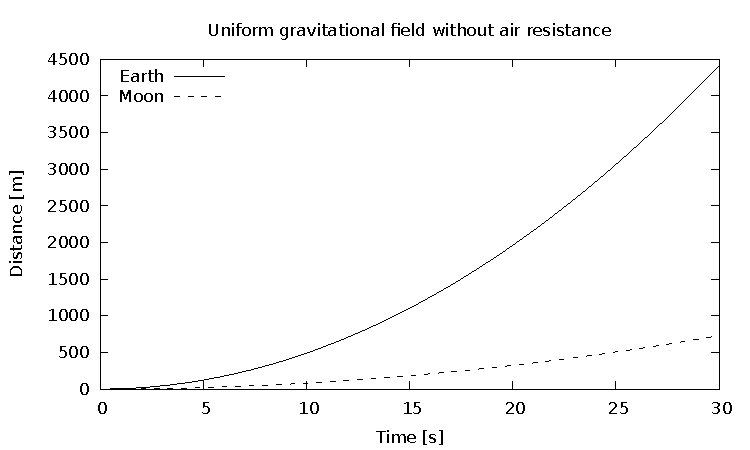
\includegraphics{gnuplot-bw}
% 	\caption{Cernobílá varianta obrázku generovaného programem Gnuplot}\label{fig:gnuplot-bw}
% \end{figure}
% 
% \begin{figure}\centering
% 	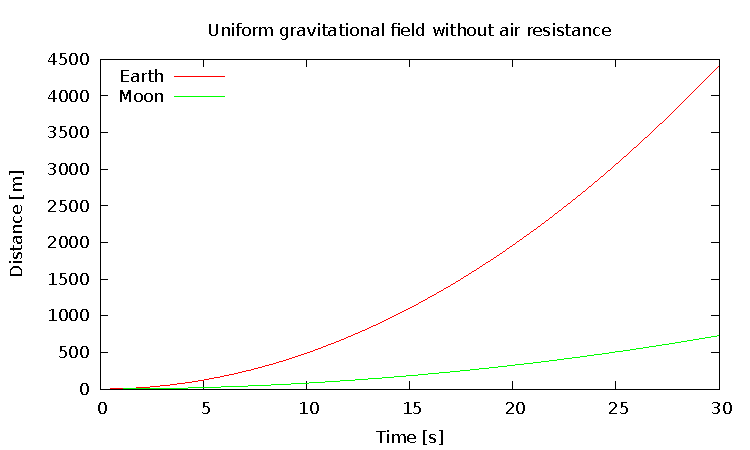
\includegraphics{gnuplot-col}
% 	\caption{Barevná varianta obrázku generovaného programem Gnuplot}\label{fig:gnuplot-col}
% \end{figure}
% 
% 
% \subsection{Tabulky}
% 
% Tabulky lze zadávat ruzne, napr. v~prostredí \verb|tabular|, avšak pro jejich vkládání platí to samé, co pro obrázky -- použijte plovoucí prostredí, v~tomto prípade \verb|table|. Napríklad tabulka \ref{tab:matematika} byla vložena tímto zpusobem.
% 
% \begin{table}\centering
% 	\caption[Príklad tabulky]{Zadávání matematiky}\label{tab:matematika}
% 	\begin{tabular}{|l|l|c|c|}\hline
% 		Typ		& Prostredí		& \LaTeX{}ovská zkratka	& \TeX{}ovská zkratka	\tabularnewline \hline \hline
% 		Text		& \verb|math|		& \verb|\(...\)|	& \verb|$...$|		\tabularnewline \hline
% 		Displayed	& \verb|displaymath|	& \verb|\[...\]|	& \verb|$$...$$|	\tabularnewline \hline
% 	\end{tabular}
% \end{table}
% 
% % % % % % % % % % % % % % % % % % % % % % % % % % % % 

\chapter{Obsah priloženého CD}

%upravte podle skutecnosti

\begin{figure}
	\dirtree{%
		.1 readme.txt\DTcomment{strucný popis obsahu CD}.
		.1 exe\DTcomment{adresár se spustitelnou formou implementace}.
		.1 src.
		.2 impl\DTcomment{zdrojové kódy implementace}.
		.2 thesis\DTcomment{zdrojová forma práce ve formátu \LaTeX{}}.
		.1 text\DTcomment{text práce}.
		.2 thesis.pdf\DTcomment{text práce ve formátu PDF}.
		.2 thesis.ps\DTcomment{text práce ve formátu PS}.
	}
\end{figure}

\end{document}